\chapter{XML}
\section{Beschreibung}
XML, kurz für {\em Extensible Markup Language}, ist eine
Auszeichnungssprache zur Darstellung und zum Austausch von
\enquote{hierarchisch strukturierten Daten}\cite{wiki:de:xml}. Das
{\em Extensible Language} rührt daher, dass der Entwickler selber
definieren kann beziehungsweise muss, welche {\em Mark-up Elemente} in
dem jeweiligen Dokument erlaubt sind. XML stellt somit nur eine
Metasprache für das festlegen einer eigenen Sprache dar.

\section{Aufbau}
\lstset{language=XML, numbers=left, stringstyle=\ttfamily, frame=box,
  rulesepcolor=\color{grey}, basicstyle=\small }
\lstset{caption=XML-Dokument; Quelle:
  http://de.wikipedia.org/wiki/XML\cite{wiki:de:xml}}
\lstinputlisting{code/examples/xml.xml}

Ein XML-Dokument besteht aus genau einem Element auf oberster Ebene
und einer beliebigen Anzahl untergeordneter Elemente, die beliebig
tief verschachtelt werden können. Zu dem können einzelne Elemente auch
Attribute haben (z.\,B. \lstinline{<eintrag attribut="wert"}).
Abgesehen davon ist es üblich, in der ersten Zeile eine
XML-Deklaration anzugeben, welcher unter anderem die verwendete XML
Version und die verwendete Zeichenkodierung angibt.
\newpage
\section{Schemasprachen}
Schemasprachen dienen dazu, die Struktur von XML-Sprachen zu
beschreiben und somit anzugeben, welche Elemente wo und wie vorkommen
dürfen. Wir werden hierbei auf die zwei bekanntesten, DTD und XML-Schema, eingehen.
(\enquote{Die zwei bekanntesten sind DTD und XML Schema.}\cite{wiki:de:xml})
\subsection{DTD}
DTD, kurz für Dokumenttypdefinition, wurde zur selben Zeit wie XML
standardisiert, und somit zu einer Zeit, in der XML-Dokumente noch
größtenteils "`erzählend"' waren und nicht zum Datenaustausch dienten.
Daher ist es z.\,B. nicht möglich, zwischen Texten und Zahlen zu
unterscheiden.

\subsection{XML-Schema}
XML-Schema, oder auch XSD für XML-Schema-Definition, ist die heutige
Möglichkeit, eine XML-Sprache zu beschreiben. Sie erlaubt es,
\enquote{den Inhalt von Elementen und Attributen zu
  beschränken}\cite{wiki:de:xml}, sprich zwischen Texten, Zahlen,
Daten und ähnlichem zu unterscheiden und ist zu dem selber ein
XML-Dokument und erlaubt somit auch komplexere Beschreibungen.

\section{XPath}\label{xpath}
XPath ist eine der zahlreichen Möglichkeiten, gezielt durch ein XML
Dokument zu navigieren und ist somit für uns im Groben mit SQL zu
vergleichen. Da es in XML weder Tabellen noch Spalten oder Zeilen
gibt, ist die Art und Weise, wie einzelne Elemente ausgewählt werden,
natürlich grundverschieden von SQL.

So besteht ein XPath Ausdruck aus {\em Lokalisierungsschritten} und
{\em Prädikaten}, wobei Lokalisierungsschritte dazu dienen, durch den
Baum zu navigierend und dabei mindestens eins, unter Umständen eine
Menge von Elementen zu selektieren. Mittels Prädikaten wird die
Auswahl weiter eingegrenzt, in dem zum Beispiel die Textnodes, sprich
die "`Werte"' der Elemente, überprüft werden.

So wäre ein simples Beispiel die Auswahl aller Produkte, die 10 Euro
oder mehr kosten. Gegeben sei folgendes Dokument:

\lstset{
  language=XML,
  numbers=left,
  stringstyle=\ttfamily,
  frame=box,
  rulesepcolor=\color{grey},
  basicstyle=\small,
  caption=
}

\lstinputlisting{code/examples/xpath.xml}

\lstset{language=XSLT}

So würde folgender XPath Ausdruck alle Produkte mit dem Preis von 10
Euro (in unserem Fall genau ein Produkt) liefern:
\lstinline{//product[price = 10]} -- Hierbei bedeutet
\lstinline{//product} soviel wie "`alle Unterelemente mit dem Namen
product"' und \lstinline{price = 10} überprüft, ob in den gefundene
Elementen ein {\em price} mit dem Wert {\em 10} vorhanden ist.
Eine Tabelle mit allen Achsen findet sich im Anhang auf Seite \pageref{table-axes}

\section{PHP}\label{xml-php}
Für uns von besonderem Interesse ist es natürlich, wie wir auf
einfache Art und Weise per PHP auf unsere XML Dateien zugreifen und
diese verwenden können. Hierfür gibt es seit PHP 5 einige
überarbeitete APIs\footnote{application programming interface} (vgl.
\enquote{PHP5 includes totally rewritten and new extensions, including
  the SAX parser, the DOM, SimpleXML, XMLReader, XMLWriter, and the
  XSLT processor. All these extensions are now based on the
  libxml2.}\cite{www:ibm:xml}), wovon vor allem zwei beliebt sind
(\enquote{Of the many APIs available in PHP5, the DOM and SimpleXML
  are the most familiar,}\cite{www:ibm:xml}). Und auf genau diese
beiden, DOM und SimpleXML werde ich im Näheren eingehen.
\newpage
\subsection{DOM}
Das {\em Document Object Model}, kurz DOM, ist ein W3C\footnote{World
  Wibe Web Consortium} Standard für das Verarbeiten und Manipulieren
von HTML und XML-Dokumenten. Dabei wird das jeweilige Dokument als
(Stamm)Baum dargestellt und behält somit den logischen Aufbau des
Ausgangsdokumentes bei. Hierbei ist zu beachten, dass DOM ein
sogenannter {\em tree-based} Parser ist und somit einen Baum vom
ganzen Dokument erstellt. Daher ist es eher ungeeignet, um große
Dokumente zu verarbeiten, da dies sonst viel Systemspeicher
beanspruchen würde (\enquote{Because DOM builds a tree of the entire
  document, it uses a lot of memory and processor time. Therefore,
  performance issues make it impractical to parse large documents with
  DOM.}\cite{www:ibm:xml}). Nichts desto trotz ist es generell die
bevorzugte Methode, um SGML/XML-Dokumente zu verarbeiten, wenn das
Hauptaugenmerk auf einem einfachen Interface liegt.
\begin{figure}[hb]
  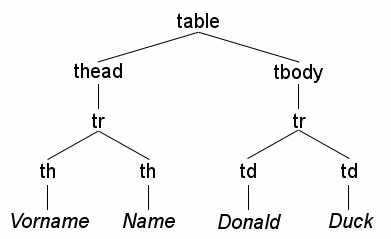
\includegraphics[width=0.5\textwidth]{images/dom}
  \caption{Der Baum einer einfachen (X)HTML Tabelle\cite{wiki:de:dom}}
\end{figure}

\subsection{SimpleXML}
SimpleXML ist eine Erweiterung, die mit PHP 5 eingeführt wurde und
unter PHP Programmierern als die einfachste Möglichkeit gilt, mit
kleinen und simpleren XML-Dokumenten zu arbeiten. Hierbei liest
SimpleXML das Dokument ein und stellt dem Entwickler ein Objekt zur
Verfügung, welches Zugriff auf die einzelnen Elemente erlaubt.
Erwähnenswert ist hierbei, dass SimpleXML in der Lage ist, mittels DOM
die Dokumente auch zu manipulieren und dank XPath eine einfache
Methode liefert, um durch das Dokument zu navigieren (vgl. Abschnitt
\ref{xpath}, Seite \pageref{xpath}).

\section{Vergleich mit relationalen Datenbanken}\label{relational_databases}
Im Folgenden werde ich XML gestützte Datenbanken mit relationalen
Datenbanken, in diesem Fall MySQL, vergleichen und schauen, inwiefern
man XML als Ersatz für solche hernehmen kann, oder ob wir es doch mit
grundlegend verschiedenen Dingen zu tun haben.

Die Merkmale einer relationalen Datenbank sind, dass sie in Tabellen
unterteilt ist, welche Zeilen (Einträge) und Spalten (Attribute)
beinhaltet. Des Weiteren ist ein Hauptmerkmal, dass Datensätze bzw.
Tabellen miteinander verknüpft werden können. Auch deswegen ist es
notwendig, dass jeder Eintrag genau identifiziert werden kann, zum
Beispiel mittels einer ID.

Dies ist in XML nicht der Fall. Zwar ist es möglich, selber Elemente
für IDs einzubringen, aber dies würde eher einem hohen Aufwand
entsprechen, wäre unter Umständen nicht eindeutig und vor allem ein
Verlinken wäre mit heimischen Mitteln nicht notwendig. Stattdessen
müsste man mit unzähligen XPaths oder XQueries oder ähnlichem
arbeiten.

Ein weiterer Unterschied ist, dass es in Datenbanken festgelegte
Datentypen gibt. So wird klar zwischen Zahlen, Strings, Daten, BLOBs
und so weiter unterschieden. Zwar ist es dank XML-Schema auch in XML
möglich, nur bestimmte Typen zuzulassen, jedoch unterliegt dies in
keiner Weise einem Standard. So könnte z.\,B. jeder eine andere Vorstellung
von einem Datum haben.

Als letztes ist noch ganz klar die Performance zu nennen. Relationale
Datenbanken unterstützen meist einen Index, welcher eine etwaige Suche
um ein vielfaches beschleunigt. Auch können die Daten effizienter und
platzsparender gespeichert werden, da nie erwartet wird, dass die
Dateien menschenlesbar sind, im Gegensatz zu XML.

Als Fazit kann man sagen, dass XML kaum bis gar nicht mit relationalen
Datenbanken wie MySQL zu vergleichen sind und im großen Maßstab sich
wohl auch nicht rechnen würden. Stattdessen ist das Einsatzgebiet eher
im Austausch von kleinen Datenmengen zu sehen, wie er z.\,B. in
modernen Webanwendungen anzutreffen ist.